\scanpage{5}
$\varphi:X\longrightarrow Y$\qquad $\varphi$ ouvert $\overset{\mathrm{déf}}\Longleftrightarrow$ ($U$ ouvert de $X\Rightarrow\varphi(U)$ ouvert)
\[
\Longleftrightarrow\deleted{\unsure{\forall}}\ (\forall B\subset Y,\quad\varphi^{-1}(\overline B)=\overline{\varphi^{-1}(B)})
\qquad(\text{NB }\subset\text{ est l'essentiel})
\]
i.e. $\forall x\in X$, $\varphi(x)\in\overline B\Rightarrow x\in\deleted{\unsure{\varphi^{-1}}}\overline{\varphi^{-1}(B)}$
i.e. $\forall\underset{\mathrm{ouv.}}{U}\ni x$, $U\cap\varphi^{-1}(B)\ne\phi$ i.e.
\[
\forall U\in\operatorname{Ouv}(x),\quad\varphi(U)\cap B\ne\phi
\qquad\text{i.e. }\forall(B\in\mathcal P(Y),x\in X,U\in\operatorname{Ouv}_x(X),)
\]
\[
\varphi(x)\in\overline B\Rightarrow\varphi(U)\cap B\ne\phi\quad\text{i.e.}\quad
\forall(U\in\operatorname{Ouv}(X))\ \forall(y\in\overset{V=}{\varphi(U)},\ B\subset Y),
\]
\[
y\in\overline B\Rightarrow V\cap B\ne\phi\quad\text{i.e.}\quad
\underbrace{V\cap B=\phi}_{B\subset X\setminus V}\Rightarrow\overline B\not\ni y
\]

\par\noindent\rule{0.95\linewidth}{0.4pt}\par

5) Les conditions 1° et 2°) sont stables par image inverse
par $X'\longrightarrow X$, mais pas 3°) bien sûr (pas $=$ pour
un plongement ouvert), ni 4°) (mais au moins
4°) est stable par induction sur un ouvert). Les
relations d'équivalences ouvertes, par contre, s'indui-
sent bien sur un ouvert (mais on rapetisse $I$
en principe). \deleted{Admettons que \unsure{l'on ait pris la même}
\unsure{pour l'un et} 1° 2° (3° bis), \unsure{et alors}\inserted{3° bis} $\forall i,j\in I$, $X_i\subset X_j$
$\Rightarrow i\leq j$}
La condition \inserted{3° bis (en présence de 1° et 2°)}
implique que la ``fidélité'' : $X_i\subset X_j\Rightarrow i\leq j$ (i.e. l'
ordre de $I$ est l'inclusion des $X_i$). \deleted{$I$ \unsure{l'inclusion}}
\deleted{\unsure{Si on a la fidélité, au contraire,} $X_i^*=\phi$ i.e. $X_i=\bigcup_{j<i}X_j$}
n'est pas vrai, exemple $I=$
\diagram{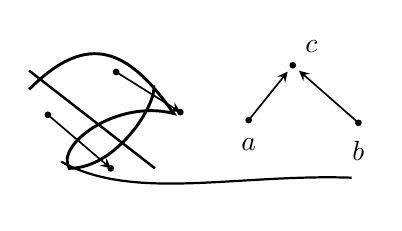
\begin{tikzpicture}[x=1.7cm,y=1.7cm,>=stealth]
\coordinate (dl) at (-1.50,.04);
\coordinate (du) at (-.99,.36);
\coordinate (dr) at (-.51,.06);
\coordinate (dd) at (-1.03,-.36);
\draw[->,line width=.6pt] (dl) -- (dd);
\draw[->,line width=.6pt] (du) -- (dr);
\foreach \p in {dl,du,dr,dd}{\fill (\p) circle (.025);}
\draw[line width=1.05pt] (-1.64,.23) .. controls (-1.19,.68) and (-.89,.52) .. (-.56,.05)
 .. controls (-.99,.16) and (-1.45,-.19) .. (-1.34,-.36)
 .. controls (-.98,-.36) and (-.68,.13) .. (-.71,.26);
\draw[line width=.9pt] (-1.64,.37) -- (-.70,-.36);
\draw[line width=.8pt] (-1.40,-.31) .. controls (-.86,-.61) and (-.09,-.40) .. (.77,-.43);
\coordinate (a) at (0,0);
\coordinate (b) at (.82,-.02);
\coordinate (c) at (.33,.41);
\draw[->,line width=.6pt,shorten >=3pt] (a) -- (c);
\draw[->,line width=.6pt,shorten >=3pt] (b) -- (c);
\foreach \p in {a,b,c}{\fill (\p) circle (.025);}
\node[below=3pt] at (a) {$a$};
\node[below=3pt] at (b) {$b$};
\node[above right=1pt] at (c) {$c$};
\end{tikzpicture}}
$X_c=X=X_a\amalg X_b$, \deleted{\unsure{tous les}} avec $X_a,X_b\ne\phi$, alors \unsure{on a}
fidélité, \inserted{les $X_i\ne\phi$,} mais $X_c^*=\phi$.

On suppose désormais 1°) 2°) 3° bis). Si $U\subset X$
est ouvert, les \inserted{$i\in I$ tels que} $X_i\cap U=U_i$ \deleted{tels que} \inserted{$\ne\phi$} forment un
ouvert $I_U$ de $U$, et \unsure{\deleted{\illegible{1}}|---} $(U_i)_{i\in I_U}$ est une
stratification ps-fidèle de $U$. (Si on part d'une
stratification stricte, on aura une stratification
stricte de $U$). Ainsi, les strat. ps. fidèles des
ouverts de $X$ forment un préfaisceau, dont les
sections sont appelées les stratifications locales
\margin{\unsure{des}}

\deleted{Supposons} \inserted{Soit} $J$ tel que $X_J$ fermé, $J$ non fermé. \inserted{Supposons $J$ minimal}
\deleted{Donc $\exists j\in J$ tel que
$\overline j\not\subset J$. Soit $j$ minimal parmi ces éléments \unsure{de $I$}
$j\in J$, $\overline j\not\subset J$, et $i<j$, $\unsure{\Longleftrightarrow|\Longrightarrow} i\in J\Rightarrow\overline i\subset J$,
\deleted{\unsure{Plus généralement}} \uline{Soit}
\deleted{$\unsure{\overline j\cap J}=\unsure{}% crossed token, no recoverable candidate; crops/150_scan005_P18.png
\unsure{\{j\}}\cup\bigcup i$}
$\unsure{J'_1}=\overline j\cap J$, donc $X_{\unsure{J'_1}}^*=X_{\overline j}^*\cap X_J^*$
est fermé, alors que $J'$ n'est pas fermé. $J'$ \unsure{un}}

parmi de tels $J$ (on suppose $I$ fini, pour simplifier\inserted{$\subset I$}) \unsure{l'on|l'un}
pour tt $K\subset I$, $K$ fermé et $K\cap J$ non fermé, \ldots $K\supset J$.
En particulier, $\forall j\in J$ tel que $\overline j\not\subset J$, \ldots $J\subset\overline j$
i.e. $j$ est plus grand él. de $J$. Donc $J$ a un plus grand
él. $j$, tel que pour tt autre élément \inserted{$j'$} de $J$, on ait
$\overline{j'}\subset J$. Donc \deleted{$\unsure{J}$}
$J_0=J\setminus\{j\}=\bigcup_{j'\in J\setminus\{j\}}\overline{j'}$ est fermé.
Donc $J=J_0\cup\{j\}$, $J_0$ fermé, $\unsure{\exists|\mathrm{et}}$ $J_0\subset\overline j$, $j\in I\setminus J_0$
$\exists i\in I\setminus J_0$ avec $i<j$. \deleted{$i\in\unsure{\overline j\cap I}$} On a donc
\[
X_J^*=X_{J_0}^*\cup X_j^*\quad(\text{réunion disjointe})
\]
qui est fermé, d'où
\[
X_j^\bullet\overset{\mathrm{déf}}=\overline{X_j^*}\setminus X_j^*\subset X_{J_0}^*=X_{J_0}=\deleted{\unsure{\mathrm{ens}}}\bigcup_{i\in J_0}X_i,
\]
sans qu'on ait
pour autant $\overline j\subset J_0\cup\{j\}$.

Soit $I'$ une partie \uline{fermée} de $I$, minimale pour la
propriété : $\exists J\subset I'$, $J$ non fermé, avec $X_J$ fermé. Soit, pour
$I'$ fini, $J$ une \deleted{\unsure{partie}} de $I'$ minimale pour les propriétés précédentes,
On a donc $J\ne\phi$ et $J=J_0\cup\{j\}$, \deleted{$\unsure{\exists}$} $J_0$ fermé, $j\notin J_0$,
\deleted{$\unsure{\overline j\not\ni i}$} $J\subset\overline j$, $\overline j\not\subset J$ \unsure{ceci|ce}, i.e. l'inclusion
\[
J=J_0\cup\{j\}\subset(\overbrace{J_0}^{\subset\overline j}\cup\overline j=\deleted{\unsure{\overline j}}\overline j)
\]
est stricte. \deleted{\unsure{de $I'$}} Pour tte
partie. Comme \inserted{\unsure{tt}} $\overline J\setminus\{j\}$ est encore fermé, d'après la condition
minimale de $I'=\overline J$ il s'ensuit que pour
 tt $J'\unsure{\subset|\in} I'\setminus\deleted{\unsure{\{i\}}}\{j\}$, $X_{J'}^*$ fermé $\Rightarrow J'$ fermé. \deleted{\unsure{En}}

\figure{\begin{tikzpicture}[x=.55cm,y=.55cm]
\foreach \x/\y in {1.87/.61,2.46/.15,2.95/.84,3.54/.96,3.27/-.13,4.10/.51,4.74/1.85,5.79/1.63,5.49/1.34,6.73/2.01,7.77/1.15,7.57/.54,8.66/.93,9.37/.58,9.66/.15,8.92/-.02,9.48/-.13}{\fill (\x,\y) circle (.055);}
\draw[line width=.9pt] (4.10,1.50)
 .. controls (3.98,1.92) and (4.18,2.22) .. (4.70,2.37)
 .. controls (5.40,2.39) and (5.94,2.23) .. (6.33,1.60)
 .. controls (6.41,1.45) and (6.11,1.35) .. (6.13,1.07)
 -- (5.90,1.03)
 .. controls (6.19,.68) and (5.95,.58) .. (5.60,.60)
 -- (5.07,.62)
 .. controls (4.80,.62) and (5.00,.94) .. (4.93,1.13)
 .. controls (4.73,1.30) and (4.33,1.26) .. (4.20,1.34)
 -- cycle;
\node[above right=1pt] at (6.73,2.01) {$j$};
\node at (.80,-.53) {$J_0$};
\end{tikzpicture}}

\deleted{particulier, pour tte partie fermée}
3 conditions équiv. :

a) $X_J^*$ fermé $\Rightarrow J$ fermé

b) $X_L^*$ ouvert $\Rightarrow L$ ouvert

c) $(\underbrace{X_j^\bullet\overset{\mathrm{déf}}=\overline{X_j^*}\setminus X_j^*\subset X_{J_0},\ J_0\text{ fermé}}_{X_{J_0\cup\{j\}}^*\text{ fermé}})
\Rightarrow\overline j\subset J_0\cup\{j\}$
(i.e. $J_0\cup\{j\}$ fermé)
(\uline{NB} \unsure{ssi} $J_0\subset\overline j$), et pour pour
$J'\subset\overline j\setminus\{j\}$, $X_{J'}^*$ fermé $\rightarrow J'$ fermé

\margin{4}
